\documentclass{standalone}
% Setup project name HERE
\newcommand{\project}{CoRed\textit{OS}}

\usepackage{tikz}
\usetikzlibrary{positioning,arrows,shapes,calc, fit, backgrounds, matrix}
\newcommand{\foldedpaper}[2][1]{
    \begin{scope}[scale=#1,line width={#1*1pt}]
        \pgfmathsetmacro{\a}{1.41}
        \pgfmathsetmacro{\b}{0.34}
        \pgfmathsetmacro{\c}{0.1}
        \pgfmathsetmacro{\d}{0.03}
        \draw         (0,0)
                --  ++(-1,0) 
                --  ++(0,\a)
                --  ++(1-\b,0)
                --  ++(\b,-\b)
                -- cycle;
        \foreach \y in {1,...,3}{
            \draw (-1+\c,{\y*\a/7+\d}) -- (-\c,{\y*\a/7+\d});
        }
        \draw[fill=white] (0,\a-\b) -- ++(-\b,0) -- ++ (0,\b);
        \node at (-0.5,0.8){#2};
    \end{scope}
}

% correct bad hyphenation here
\hyphenation{
  semi-conduc-tor
  OSEK
  AUTOSAR
  CoRed
}

\usepackage{xcolor}
\usepackage{graphicx}

% Colors
\definecolor{i4red}{rgb}{0.69,0.11,0.18}
\definecolor{i4blue}{rgb}{0.0,0.4,0.62}
\definecolor{i4gray}{rgb}{0.827,0.827,0.827}

% PDF
\usepackage[pdftex,%
    bookmarks = false, % IEEE Explore does not want bookmarks
    ]{hyperref}
\hypersetup{%
    %draft = true, % IEEE Explore does not want links draft, disables all hypertext options
    colorlinks = true,
    linkcolor = black,
    anchorcolor = black,
    citecolor = black,
    filecolor = black,
    urlcolor = black,
    pdftitle = {dOSEK: A Dependable RTOS for Automotive Applications},
    %pdfsubject = {},
    pdfauthor = {Martin Hoffmann, Christian Dietrich, Daniel Lohmann}
    pdfkeywords = {CoRed, Operating Systems, Embedded Systems, Real-Time Systems, Dependability, Safety, OSEK, AUTOSAR, Coded Processing, Transactional},
    pdfcreator = {},
    pdfproducer = {},
}
\usepackage{acronym}
\acrodef{ECU}{electronic control unit}
\acrodef{cored}[\textit{CoRed}]{\textit{Combined Redundancy}}
\acrodef{EAN}{\textit{Extended AN Code}}
\acrodef{SOR}[SOR]{sphere of replication}
\acrodef{SPOF}{single point of failure}
\acrodef{OS}{operating system}
\acrodefplural{SPOF}[SPOFs]{single points of failure}
\acrodef{VCP}{vital coded microprocessor}

\begin{document}


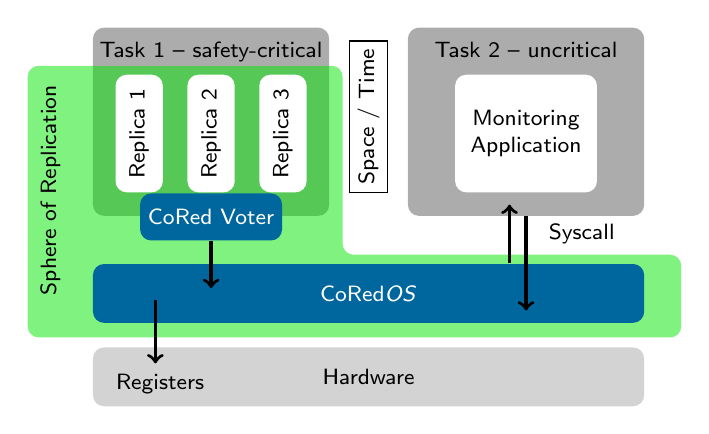
\begin{tikzpicture}
\pgfdeclarelayer{background}
\pgfdeclarelayer{foreground}
\pgfsetlayers{background,main,foreground}

\sffamily
\footnotesize
\tikzstyle{basenode}=[rounded corners, align=center];
\tikzstyle{proj}=[basenode, white, fill=i4blue,minimum height=2.5em, minimum width=7cm];
\tikzstyle{hw}=[basenode,  fill=i4gray,minimum height=2.5em, minimum width=7cm];
\tikzstyle{sysc}=[basenode, minimum height=0.5cm, text width=1cm, node distance=2em]
\tikzstyle{task}=[basenode,  fill=gray!65,minimum height=8em, minimum width=3cm, node distance=3em];
\tikzstyle{thread}=[basenode, fill=white,];
\tikzstyle{threaduns}=[basenode,  fill=white,minimum height=5em, minimum width=1.8cm];
\tikzstyle{threadrep}=[basenode,  fill=white,minimum height=5em, minimum width=0.6cm, node distance=1em];
\tikzstyle{voter}=[basenode, white, fill=i4blue,  minimum width=1.6cm, minimum height=2em];
\tikzstyle{sor_tmr}=[fill=green!90!black, fill opacity=0.5, minimum width=1cm, minimum height=7.8em];
\tikzstyle{basearr}=[very thick, black];
\tikzstyle{arr}=[basearr, ->];
\tikzstyle{revarr}=[basearr, <-];
\tikzstyle{proj_sor}=[fill=green!90!black, fill opacity=0.5, draw=none];
\tikzstyle{ext_arr}=[-open triangle 90 ,line width=0.1cm,color=green!80!black,cap=round,join=round];

\node[proj](pr){\project{}};
\node[ hw, below = 1em of pr](hw){Hardware};

\begin{scope}[on background layer]
\node[ task, above=2em of pr.north west, anchor=south west ](task1){x};
\node[ task, above=2em of pr.north east, anchor=south east ](task2){x};
\end{scope}

\node[ below = 0.3em of task2.north ] {Task 2 -- uncritical};
\node[ threaduns, below = 2em of task2.north] () {Monitoring\\ Application};

\node[ below = 0.3em of task1.north ] {Task 1 -- safety-critical};

\node[ threadrep, below = 2em of task1.north] (rep2) {\rotatebox{90}{Replica 2}};
\node[ threadrep, left = of rep2] (rep1) {\rotatebox{90}{Replica 1}};
\node[ threadrep, right = of rep2] () {\rotatebox{90}{Replica 3}};
\node[ voter, below=0em of rep2.south](voter){CoRed Voter};

\node[ draw, above=3em of pr.north]{\rotatebox{90}{Space / Time}};
%\node[ above = 0.6em of pr.172,](syscc){Syscall};
\node[ above = 0.5em of pr.8,](syscc1){Syscall};

\node[ left=1em of task1.210]{\rotatebox[]{90}{Sphere of Replication}};

\draw[ arr ] (voter.south) -- +(0,-2em);
\draw[ arr ] (task2.south) -- +(0,-4em);
\draw[ arr ] (pr.12) -- +(0,2.5em);

\node[ sysc, below  = 1.7em of pr.-172, minimum width=2cm](regi){Registers};
\draw[ revarr ] (regi.north) -- +(0,0.8cm);

\begin{scope}[on background layer]
\node[left= 3em of rep1.north west](sst){};
\filldraw[ proj_sor, rounded corners] (sst.north west) -- ++(4cm,0) -- ++(0,-2.4cm) -- ++(4.3cm,0) -- ++(0,-1.05cm) -- ++(-8.3cm,0) -- cycle;
\end{scope}

\end{tikzpicture}

\end{document}
